\documentclass[12pt,a4paper]{article}

\usepackage[utf8]{inputenc}
\usepackage[english]{babel}
\usepackage{amsmath}
\usepackage{amsfonts}
\usepackage{amssymb}
\usepackage{graphicx}
\usepackage{booktabs}
\usepackage[super,sort&compress,numbers]{natbib}
\usepackage{hyperref}
\usepackage{url}
\usepackage{indentfirst}

\setlength{\parindent}{1.5em}
\setlength{\parskip}{0pt}

\title{\Large Reinforcement Learning for Autonomous Driving: Efficiency and Comfort Optimization}
\author{Anrui Wang}
\date{\today}

\begin{document}
\sloppy

\maketitle

\begin{abstract}
    
\end{abstract}

\textbf{Keywords:}~Reinforcement Learning, Autonomous Driving, Multi-Objective Optimization, Efficiency, Comfort\hfill\null

\section{Introduction}

\subsection{Background and Current Research Status}
Deep Reinforcement Learning (RL) has become a significant research domain in autonomous driving. Modern RL algorithms effectively learn complex driving policies in high-dimensional environments like traffic simulators\cite{jin2025}, with applications spanning lane keeping, adaptive cruise control, intersection navigation, and overtaking maneuvers.

Early research established the viability of RL for vehicle control, with the Deep Deterministic Policy Gradient (DDPG) algorithm enabling human-comparable steering and acceleration capabilities\cite{zhu2020}. Subsequent studies have focused on singular objectives: safety (collision avoidance) or efficiency (minimizing travel time or fuel consumption). For example, a Proximal Policy Optimization (PPO)-based controller improved fuel economy by 17\% over human baselines while maintaining comparable travel times\cite{zhu2021}, while safety-optimized policies have produced extended accident-free operation\cite{survey2023}.

Driving, however, inherently involves trade-offs among multiple objectives—time efficiency, energy conservation, safety, and passenger comfort. Recent research has begun incorporating multiple objectives within RL frameworks, recognizing that truly human-like autonomous driving must simultaneously optimize efficiency, safety, and comfort parameters.

\subsection{Research Gaps and Challenges}
While the application of optimization techniques, particularly single-objective methods within RL, has shown considerable progress in specific aspects of autonomous vehicle control such as trajectory planning or velocity control \cite{survey2023, kiran2022, lillicrap2016}, a significant research gap persists concerning the holistic treatment of multiple, often conflicting, performance criteria. Driving inherently necessitates balancing diverse objectives including, but not limited to, time efficiency, energy consumption, safety margins, and passenger comfort \cite{he2023}. However, much of the existing literature tends to simplify the problem by focusing on optimizing a singular objective, such as minimizing travel time or maximizing fuel economy \cite{zhu2021, he2023}, or by prioritizing safety above all else \cite{zhu2021}.

Consequently, the development of sophisticated multi-objective optimization (MOO) frameworks tailored for autonomous driving control remains an open and critical challenge \cite{survey2023}. Effectively and simultaneously optimizing competing objectives like operational efficiency and passenger comfort, which often exhibit inverse relationships, requires methodologies capable of navigating complex trade-offs. Although nascent approaches in Multi-Objective Reinforcement Learning (MORL) are emerging \cite{li2019, yang2019, zhang2023, jin2025, selvaraj2023}, many existing strategies either aggregate multiple criteria into a single scalar reward function, potentially obscuring important trade-offs, or employ hierarchical or lexicographical methods that impose fixed priorities \cite{li2019, zhang2023}. This underscores the pressing need for advanced MOO techniques within RL that can generate diverse sets of optimal policies reflecting different balances between objectives like efficiency and comfort, thereby motivating the research presented in this work.

\section{Related Work}

\subsection{Deep RL Algorithms}
Various RL algorithms have been applied to autonomous driving, each with distinct advantages. As documented by Kiran et al.\cite{kiran2022}, value-based methods like Deep Q-Networks (DQN) operate in discrete action spaces and have been implemented for basic driving tasks\cite{hossain2023}. Sallab et al.\cite{sallab2016} demonstrated end-to-end RL for lane-keeping from visual input, though discrete actions limit the fine control needed for passenger comfort.

Policy gradient and actor-critic methods better suit continuous control scenarios. DDPG generates continuous commands and has been widely used for smooth control applications. Zhu et al.\cite{zhu2020} applied DDPG to adaptive cruise control, showing improved safety margins and reduced acceleration variations, enhancing both comfort and safety compared to conventional controllers. PPO has been valued for its training stability, with applications in eco-driving using Long Short-Term Memory (LSTM) networks to optimize velocity profiles\cite{zhu2021}. Soft Actor-Critic (SAC), which balances reward and entropy, offers sample-efficient learning for high-dimensional tasks.

Recent advances include hybrid architectures integrating discrete and continuous control. Jin et al.\cite{jin2025} proposed a framework handling both lane changes (discrete) and steering/acceleration (continuous) simultaneously. Generally, actor-critic algorithms are preferred for comfortable driving as they enable the fine-grained control essential for passenger comfort, with DDPG\cite{lillicrap2016} being particularly influential.

\subsection{Model-based and Hybrid Approaches}
To address sample inefficiency and incorporate physical knowledge, researchers have explored model-based approaches. Zhu\cite{zhu2021} developed Safe Model-Based Off-Policy RL (SMORL), integrating vehicle dynamics models and safety checkers into training. Another direction combines RL with classical controllers, such as pairing RL with Model Predictive Control (MPC) for intersection navigation—RL handling high-level decisions and MPC managing low-level control\cite{survey2023}.

Multi-Objective Reinforcement Learning (MORL) effectively balances competing objectives. Li and Czarnecki\cite{li2019} introduced thresholded lexicographic Q-learning, prioritizing safety before comfort and progress. Yang et al.\cite{yang2019} developed a generalized MORL algorithm adapting to different objective preferences, approximating the Pareto frontier of optimal driving behaviors. Zhang et al.\cite{zhang2023} applied lexicographic actor-critic methods to urban driving, while He and Lv\cite{he2023} focused on energy efficiency alongside safety. While model-free approaches dominate current research, these model-based and hybrid methods are increasingly valuable for multi-objective optimization.

\subsection{Frameworks and Simulation Environments}
RL can be implemented at various levels of the driving stack. End-to-end approaches map sensor inputs directly to vehicle commands but face challenges with high-dimensional observations and interpretability\cite{survey2023}. Kendall et al.\cite{kendall2019} achieved the first real-world end-to-end driving using monocular camera input. Alternative approaches use mid-level state representations, simplifying learning and improving sample efficiency\cite{survey2023}. Xu et al.\cite{xu2018} modeled highway driving as a Markov Decision Process (MDP) with dedicated reward components and deployed their policy on real vehicles. Selvaraj et al.\cite{selvaraj2023} developed a framework explicitly addressing efficiency, safety, and comfort through an integrated co-simulation platform.

Due to safety concerns with real-world testing, researchers rely on high-fidelity simulators. CARLA\cite{pmlr-v78-dosovitskiy17a} provides realistic urban environments and sensor streams for RL research. MetaDrive\cite{metadrive} facilitates research through procedurally generated roads, demonstrating that diverse training environments improve zero-shot performance on unseen conditions. Simulation of Urban Mobility (SUMO)\cite{lopez2018} enables traffic-level simulations where RL agents control individual vehicles among many. Researchers sometimes combine simulators—Selvaraj et al.\cite{selvaraj2023} created a co-simulation framework linking traffic simulation, network communication, and vehicle dynamics models.

In the typical RL framework, an agent observes the current state (vehicle positions, velocities), selects actions (acceleration, steering), receives rewards, and transitions to the next state, repeatedly learning to maximize cumulative reward. Multi-agent settings introduce additional objectives like cooperative efficiency and fairness, though challenges remain in sample complexity, interpretability, and multi-objective optimization\cite{survey2023,kiran2022}.

\section{Methodology}
\subsection{Reward Function Design for Efficiency and Comfort}\label{sec:reward_design}

To guide the reinforcement learning (RL) agent effectively towards achieving the concurrent objectives of driving efficiency and passenger comfort, we propose a carefully structured composite reward function implemented within the MetaDrive simulation environment \cite{metadrive}. The total reward at each timestep \( t \), denoted by \( R_t \), is computed as the sum of several distinct components, each reflecting a particular aspect of desirable driving behavior. Formally, the reward function can be expressed as:
\[
R_t = w_{driving} \cdot \Delta d_{long, t} + w_{speed} \cdot \frac{v_t}{v_{max}} - w_{accel} \cdot |v_t - v_{t-1}| - P_{wrong\_way} \cdot \mathbb{I}_{wrong\_way, t} + R_{terminal, t}
\]
where \( \Delta d_{long, t} \) is the longitudinal distance covered, \( v_t \) is the current speed (\( v_{max} \) being the maximum), \( |v_t - v_{t-1}| \) is the magnitude of speed change, \( \mathbb{I}_{wrong\_way, t} \) indicates driving on a wrong-way lane, \( w_{driving}, w_{speed}, w_{accel} \) (set to 0.015) are weighting coefficients, \( P_{wrong\_way} \) is the wrong-way penalty magnitude, and \( R_{terminal, t} \) is the terminal reward or penalty applied upon episode termination (positive \( R_{success} \) for success, negative \( -P_{crash} \) for crashes, or negative \( -P_{fail} \) for other failures).

The design of \( R_t \) incorporates several key elements to shape the agent's policy. Firstly, to directly promote driving efficiency, the agent receives a positive \textit{Driving Reward} (\( w_{driving} \cdot \Delta d_{long, t} \)) proportional to the forward distance traveled along its designated navigation path during the timestep. This encourages continuous advancement towards the destination. Efficiency is further reinforced by a \textit{Speed Reward} (\( w_{speed} \cdot \frac{v_t}{v_{max}} \)), which provides a positive signal based on the vehicle's current speed relative to its maximum allowable speed. This component incentivizes maintaining appropriate speeds, discouraging excessive caution while respecting limits, thereby contributing to timely task completion.

Passenger comfort is explicitly addressed through an \textit{Acceleration Penalty} (\( -w_{accel} \cdot |v_t - v_{t-1}| \)). This term penalizes the magnitude of acceleration or deceleration, as abrupt speed changes negatively impact ride comfort due to increased jerk. By incorporating this penalty, with \( w_{accel} \) set based on our implementation, the agent is guided towards smoother velocity profiles. Safety and adherence to traffic rules are enforced primarily through a significant \textit{Wrong-Way Penalty} (\( -P_{wrong\_way} \cdot \mathbb{I}_{wrong\_way, t} \)), applied whenever the vehicle enters a lane intended for opposing traffic flow, strongly deterring such hazardous maneuvers.

Finally, the overall task objective is reinforced by \textit{Terminal Rewards and Penalties} (\( R_{terminal, t} \)). A substantial positive reward (\( R_{success} \)) is granted upon successful completion of the driving task by reaching the destination. Conversely, significant penalties are applied if the episode terminates prematurely due to collisions (\( -P_{crash} \)) or other failures like driving off-road (\( -P_{fail} \)). These terminal signals provide sparse but strong guidance, ensuring the agent prioritizes safe and successful task completion over the entire episode duration.

Synthesizing these components into the single scalar reward signal \( R_t \) allows the RL agent to learn a complex policy that effectively balances the often competing demands of driving efficiency, passenger comfort, and operational safety. This meticulously crafted reward function is therefore central to achieving reliable and desirable autonomous driving behaviors in our experiments.

\section{Experiments and Results}
\subsection{Experimental Setup}

To evaluate the effectiveness of our proposed reward function in balancing driving efficiency and passenger comfort, we conducted a series of experiments using a state-of-the-art reinforcement learning approach within a realistic simulation environment. 

The primary focus of our investigation was to analyze the impact of the acceleration penalty component within our custom reward function, as detailed in Section \ref{sec:reward_design}, on the learned driving behavior. Specifically, we systematically varied the weighting coefficient for the acceleration penalty (\(w_{accel}\) in the reward formulation) across a set of distinct values: \{0.00, 0.005, 0.01, 0.015, 0.02\}. This allowed us to observe how different levels of emphasis on penalizing abrupt acceleration and deceleration influence the trade-off between efficiency and comfort. Each weight value corresponded to a separate training run, ensuring a controlled comparison.

To assess the performance of the agents trained under these varying conditions, we employed a combination of quantitative and qualitative metrics. The learning performance during training was monitored using the mean episode reward (\texttt{rollout/ep\_rew\_mean}) logged by Stable Baselines3, providing insight into the agent's ability to maximize the cumulative reward signal over time. For evaluating the resulting driving policies, we focused on ride comfort, measured quantitatively using metrics derived from vehicle dynamics data (referred to as ``frames comfort'' in our analysis) gathered during dedicated evaluation runs. Additionally, the qualitative nature of the learned driving behavior, particularly in complex maneuvers like roundabout navigation, was assessed through visual inspection of recorded simulation sequences (e.g., the roundabout navigation GIF).


\subsection{Training Performance Analysis}

\begin{figure}[ht]
\centering
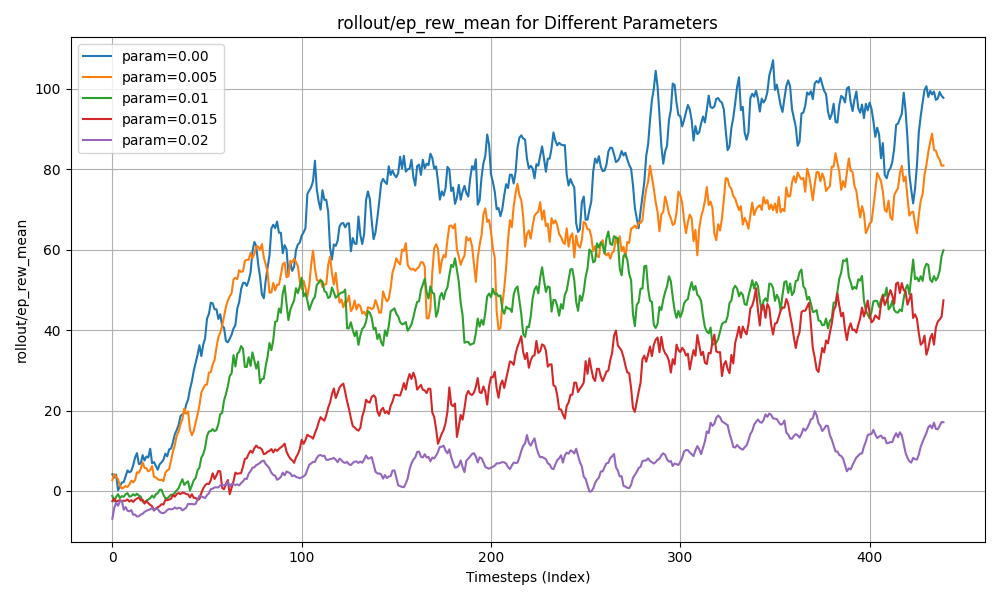
\includegraphics[width=\textwidth]{./img/output.png}
\caption{Learning progress trained with different acceleration penalty weights}
\label{fig:learning_curves}
\end{figure}

Figure \ref{fig:learning_curves} illustrates the learning progress, represented by the mean episode reward (\texttt{rollout/ep\_rew\_mean}), over the course of training for agents utilizing five different acceleration penalty weights (0.00, 0.005, 0.01, 0.015, and 0.02). All agents exhibited successful learning, as indicated by the generally increasing trend in mean episode rewards throughout the training process. While exhibiting considerable variance, the learning curves for all parameter settings appeared to approach convergence towards the end of the training period. A comparison across the different penalty weights reveals a clear impact on both learning dynamics and final performance. Increasing the acceleration penalty weight generally resulted in slower learning convergence and notably lower final mean episode rewards. Specifically, the agent trained without any acceleration penalty (weight=0.00) achieved the highest reward levels, fluctuating around a mean reward of 90-100 in the later stages of training. Conversely, the agent trained with the highest penalty weight (weight=0.02) demonstrated the slowest learning rate and converged at a significantly diminished mean reward level, approximately 10-20. The intermediate penalty weights yielded performance levels between these extremes, with final rewards generally decreasing as the penalty weight increased. This observation suggests that while the penalty term may influence agent behavior as intended, its magnitude directly impacts the maximum achievable cumulative reward, primarily due to the penalty term's direct negative contribution to the total reward calculation per episode.

\subsection{Evaluation Results}

\begin{table}[ht]
\centering
\begin{tabular}{|c|c|c|}
\hline
\textbf{Acc Penalty Weight} & \textbf{Frames} & \textbf{Comfort}  \\
\hline
0.00 & 244.09 & 21.08 \\
0.005 & 275.38 & 19.32 \\
0.01 & 246.44 & 19.73 \\
0.015 & 230.3 & 20.58 \\
0.02 & 458.24 & 9.35 \\
\hline
\end{tabular}
\caption{Evaluation metrics for agents trained with different acceleration penalty weights}
\label{tab:evaluation_results}
\end{table}

To quantitatively assess the impact of the acceleration penalty on ride comfort, the trained agents corresponding to each penalty weight were evaluated, and the results are summarized in Table \ref{tab:evaluation_results}. The 'comfort' metric reported in this table serves as a quantitative proxy for ride smoothness during these evaluations. It is understood that this metric quantifies aspects related to passenger comfort, likely derived from kinematic data such as vehicle acceleration or jerk, where lower values indicate smoother maneuvers and consequently, higher ride comfort. Examining the relationship between the acceleration penalty weight used during training and the resulting comfort metric during evaluation reveals a distinct trend. Increasing the acceleration penalty weight generally led to improved ride comfort, as indicated by lower values of the comfort metric. Although the trend exhibited some minor fluctuations for intermediate weights, the agent trained with the highest penalty (weight=0.02) achieved a significantly lower comfort metric value (9.35) compared to the agent trained without any penalty (21.08). This finding strongly suggests that the acceleration penalty component within the reward function was effective in achieving its objective. By penalizing high accelerations during the learning phase, the agent was successfully encouraged to adopt smoother driving behaviors, leading to demonstrably improved ride comfort in evaluation scenarios, particularly when a substantial penalty weight was applied.

\section{Conclusion}
% What we have done

% What we havn't done? Future work


\bibliographystyle{unsrtnat}
\bibliography{references}

\end{document}